\documentclass[12pt]{article}

\usepackage[utf8]{inputenc}
\usepackage{multicol}
\usepackage{blindtext}
\usepackage{graphicx}
\usepackage[dvipsnames]{xcolor}
\graphicspath{ {./images/} }
%\pagecolor{Periwinkle}

\title{Starport: Lending Kernel}
\author{Andrew Redden \\ \texttt{andrew@astaria.xyz}
        \and
        Joseph Delong \\ \texttt{joe@astaria.xyz}
        \and
        Gregory Curtis \\ \texttt{greg@astaria.xyz}}
\date{\today}

\begin{document}

\maketitle

\begin{abstract}
Starport is a simple kernel framework used for composing lending protocols on the Ethereum Virtual Machine (EVM).
Starport itself is not a lending protocol but instead handles the message passing and agreement enforcement that is required for any lending protocol.
Any existing or future lending protocol can be constructed by implementing the three primary Starport module interfaces \emph{Pricing}, \emph{Status}, and \emph{Settlement}.

The Starport kernel design explores loan origination as a conditional swap with modular  abstractions for settlement. Starport kernel has the capability to support collateralized loans and options for any ERC-20\cite{erc20}, ERC-721\cite{erc721}, or ERC-1155\cite{erc1155} as either collateral or debt. Rebasing tokens are not supported.
\end{abstract}

\section{Core}
The Starport kernel is supported by two core contracts \texttt{Starport} and \texttt{Custodian}.
\subsection{Starport}

\texttt{Starport} is the entry point for origination and refinancing.\\

The duty of \texttt{Starport} is to enforce the agreements \texttt{originate}, \texttt{refinance}, and to maintain the record of loan state. \texttt{Starport} manages the loan state mutations through a  \texttt{loanId}. Each loan is uniquely identified by a \texttt{loanId} that is a \texttt{keccak256} hash of the \texttt{Starport.Loan} struct.

\subsection{Custodian}

\texttt{Custodian} is the entry point for repayment or settlement.\\

The duty of the Custodian is to manage loan settlement conditions by acting as a \emph{Seaport}\cite{seaport}  \emph{ContractOfferer} . Borrower collateral is purchased from the Custodian with the terms generated by the modules.\\

Custodian is not a strict implementation, borrowers and lenders can propose differing implementations of the \texttt{Custodian} that support the \texttt{Custodian} interface. However, a gas efficient default \texttt{Custodian} contract is provided with Starport.

\section{Modules}
Modules are implementations of the module interfaces that are untrusted by the core. Each module serves a purpose within the lending lifecycle providing parameters and conditions for the core contracts to enforce.
\subsection{Pricing}
The duty of the \texttt{Pricing} module is to provide the conditions of repayment to \texttt{Custodian} and the conditions of refinance to the \texttt{Starport} contract.
\subsection{Status}
The duty of the \texttt{Status} module is to provide the status of whether a loan is active or inactive. An inactive status allows a loan to be settled by the \texttt{Custodian}.
\subsection{Settlement}
The duty of the \texttt{Settlement} module is to provide the conditions settlement to the \texttt{Custodian}.
\section{Loan Lifecycle}
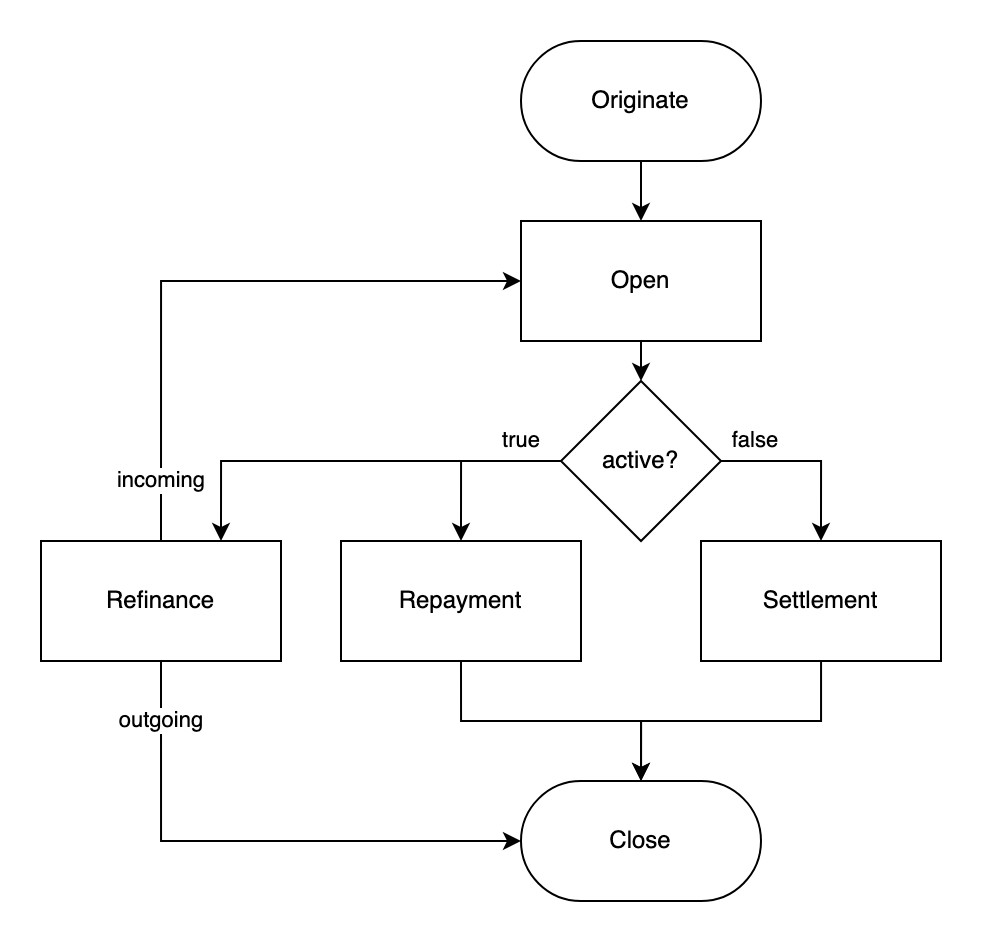
\includegraphics[width=\textwidth]{loan_lifecycle.png}

\begin{itemize}
	\item \textbf{Originate} (action)
	\begin{itemize}
		\item \texttt{Starport} loans begin in the \texttt{originate} method. 

			\texttt{Starport} enforces the transfers of the collateral from the \texttt{loan.borrower} to the \texttt{Custodian}, debt transfers from the \texttt{loan.issuer} to the \texttt{loan.borrower}, and transfers the \texttt{additionalTransfers}.\\
			When authentication conditions of the \texttt{loan.borrower} and \texttt{loan.issuer} are met, \texttt{loanId} is sent to \texttt{Open}.
	\end{itemize}
	
	\item \textbf{Open} (event)
	\begin{itemize}
		\item An \texttt{Open} event creates a new \texttt{loanId} that is hashed from the \texttt{Starport.Loan} struct, making each cryptographically unique and representing all data necessary to manage the \texttt{loanId} using off chain data availability through representment.
	\end{itemize}
	
	\item \textbf{Active} (conditional)
	\begin{itemize}
		\item Active is a conditional provided by \texttt{Status.isActive()}. When \texttt{isActive()} returns \texttt{true}, the repayment or refinance condition is allowed. When \texttt{isActive()} returns \texttt{false} the settlement condition is allowed. The transition from \texttt{isActive()} from \texttt{true} to \texttt{false} is not a immutable transition. If the condition flips from \texttt{true} to \texttt{false} it is possible for the condition to return \texttt{true} again in the future.
	\end{itemize}
	
	\item \textbf{Repayment} (action)
	\begin{itemize}
		\item Repayment condition allows the \texttt{loan.borrower} of the associated \texttt{loanId} to repay their loan through the \emph{Custodian} as a \emph{Seaport} \emph{ContractOfferer} on the conditions returned from\\ \texttt{Pricing.getPaymentConsideration()}. During which the \texttt{loan.issuer} (lender) is repaid and the \texttt{loan.originator} is paid carry (if included). Afterwards, the \texttt{loanId} is sent to \texttt{Close}.
	\end{itemize}
	
	\item \textbf{Settlement} (action)
	\begin{itemize}
		\item Settlement conditions are provided by the \texttt{Settlement} module.\\\texttt{Settlement.getSettlementConsideration()} returns the authorized and conditions of settlement. If authorized is \texttt{address(0)} any fulfiller can provide the settlement conditions, otherwise the settlement fulfiller is restricted to authorized only.
	\end{itemize}
	
	\item \textbf{Refinance} (action)
	\begin{itemize}
		\item Refinance conditions are provided by the \texttt{Pricing} module.\\\texttt{Pricing.getRefinanceConsideration()} returns the conditions of the refinance. Refinance enforces transfers from the \texttt{lender} to the outgoing \texttt{loan.issuer}, enforces carry transfers from the \texttt{lender} to the outgoing \texttt{loan.originator}, and applies those payments to the \texttt{loan.debt} array and replaces the \texttt{pricingData}. The outgoing \texttt{loanId} is sent to \texttt{Close} and an incoming \texttt{loanId} is sent to \texttt{Open}.
	\end{itemize}
	
	\item \textbf{Close} (event)
	\begin{itemize}
		\item A \texttt{Close} event deletes a \texttt{loanId} from \texttt{Starport}. A deleted \texttt{loanId} cannot be refinanced, repaid, settled, or originated.
	\end{itemize}
\end{itemize}

\section{Actors}
Within the Starport system there are three distinct actors borrowers, lenders, and fulfillers.
\begin{enumerate}
	\item \textbf{Borrower} is the user providing collateral in exchange for debt.
	\item \textbf{Lender} is the user providing debt to the borrower in exchange for future repayment (presumably with interest but module implementation is independent of this fact).
	\item \textbf{Fulfiller} is the transacting party commonly known as \emph{msg.sender}. A fulfiller can be a borrower, lender, or a different third party.
\end{enumerate}

\section{Authentication}
\subsection{Origination}
For the \texttt{originate} method, Starport will ensure that the fulfiller is authorized by both the \texttt{loan.borrower} (borrower) and the \texttt{loan.issuer} (lender).\\

There are three methods to ensure the fulfiller is authorized by the borrower and the lender.

\begin{enumerate}
	\item\texttt{msg.sender}
		\begin{itemize}
			\item\texttt{msg.sender} must be equal to either the borrower or lender
		\end{itemize}
    	
	\item approval
		\begin{itemize}
    		\item\texttt{msg.sender} is approved by the either the lender or borrower
    			\begin{itemize}
        			\item approval must be \texttt{ApprovalType.BORROWER} or \texttt{ApprovalType.LENDER}, it cannot be both
        		\end{itemize}
        \end{itemize}
	\item \texttt{CaveatEnforcer.SignedCaveats}
		\begin{itemize}
    		\item A signed struct that enforces conditional approval from either the borrower or lender
    			\begin{itemize}
        			\item Validates the signature that it is the borrower or lender
        			\item Makes an external call to a \texttt{CaveatEnforcer} with the signed in data
        		\end{itemize}
        \end{itemize}
\end{enumerate}
A fulfiller must provide at least one of the following authentication methods for both the lender and the borrower.
\subsection{Refinancing}
For the \emph{refinance} method within Starport, we need to ensure that the fulfiller is authorized by the refinancing \emph{lender}.\\

We must authenticate using one of the three methods described in the \emph{originate} section.

\section{Additional Transfers}
\texttt{additionalTransfers} is a concept within \texttt{originate} that allows the fulfiller to reimburse themselves or others for cost incurred to perform the transaction or an additional reward for executing the transaction.

\texttt{additionalTransfers} is passed to \texttt{CaveatEnforcer} and validated conditionally. For instance a borrower signs into their \texttt{SignedCaveat} an allowance for an \texttt{additionalTransfer} to reimburse the fulfiller for pre-purchasing an ERC-721.

The fulfiller provides \texttt{additionalTransfers} and the authentication model either allows the transfers or reverts.

\section{Representment}
Starport data availability and loan state mutations rely on a concept developed in Astaria v0 called \emph{representment}.

\emph{Representment} in the context of blockchains is a data availability strategy that reduces storage requirements and as an effect reduces transaction gas consumption.

All data necessary is stored in a \texttt{Starport.Loan} struct and hashed using \texttt{keccak256} into a single \texttt{bytes32} value \texttt{loanId}. Any call to the Starport or modules requires the \texttt{Starport.Loan} struct be represented, hashed and validated for an open loan before the transaction can proceed.

\begin{thebibliography}{9}
\bibitem{erc20}
Fabian Vogelsteller, Vitalik Buterin. 
\textit{ERC-20: Token Standard}. 
Ethereum Improvement Proposals, 2015.\\
https://eips.ethereum.org/EIPS/eip-20

\bibitem{erc721}
 William Entriken, Dieter Shirley, Jacob Evans, Nastassia Sachs. 
\textit{ERC-721: Non-Fungible Token Standard}. 
Ethereum Improvement Proposals, 2018.\\
https://eips.ethereum.org/EIPS/eip-721

\bibitem{erc1155}
Witek Radomski, Andrew Cooke, Philippe Castonguay, James Therien, Eric Binet, Ronan Sandford. 
\textit{ERC-1155: Multi Token Standard}. 
Ethereum Improvement Proposals, 2018.

\bibitem{seaport}
0age, stephankmin, d1ll0n, emo-eth, horsefacts. 
\textit{Seaport}. 
Github, 2022.\\
https://github.com/ProjectOpenSea/seaport

% Add more references as needed
\end{thebibliography}

\end{document}
